\section{Background}
\label{sec:background}
This section will briefly mention the background of this research, and will give a summary of the ADRIAN protocol. It will also detail the components of the ADRIAN protocol that are relevant to this research.

\subsection{ADRIAN Protocol}
\label{ssec:adrian}

As mentioned in the introduction, this research builds upon the earlier work of Z.A. Mann and S. Smolka \cite{mann2023ADRIAN}. They propose a protocol, called \ADRIAN (or ADRIAN for short), which has the core objective to identify and mitigate risks in distributed systems, leveraging a decentralized and adaptive approach. Unlike conventional security frameworks that rely on a centralized authority to oversee system security, ADRIAN empowers autonomous software agents to collaboratively assess and address security risks. An abstract representation of the ADRIAN approach is shown in Figure \ref{fig:adrian-architecture}.

\begin{figure}
    \centering
    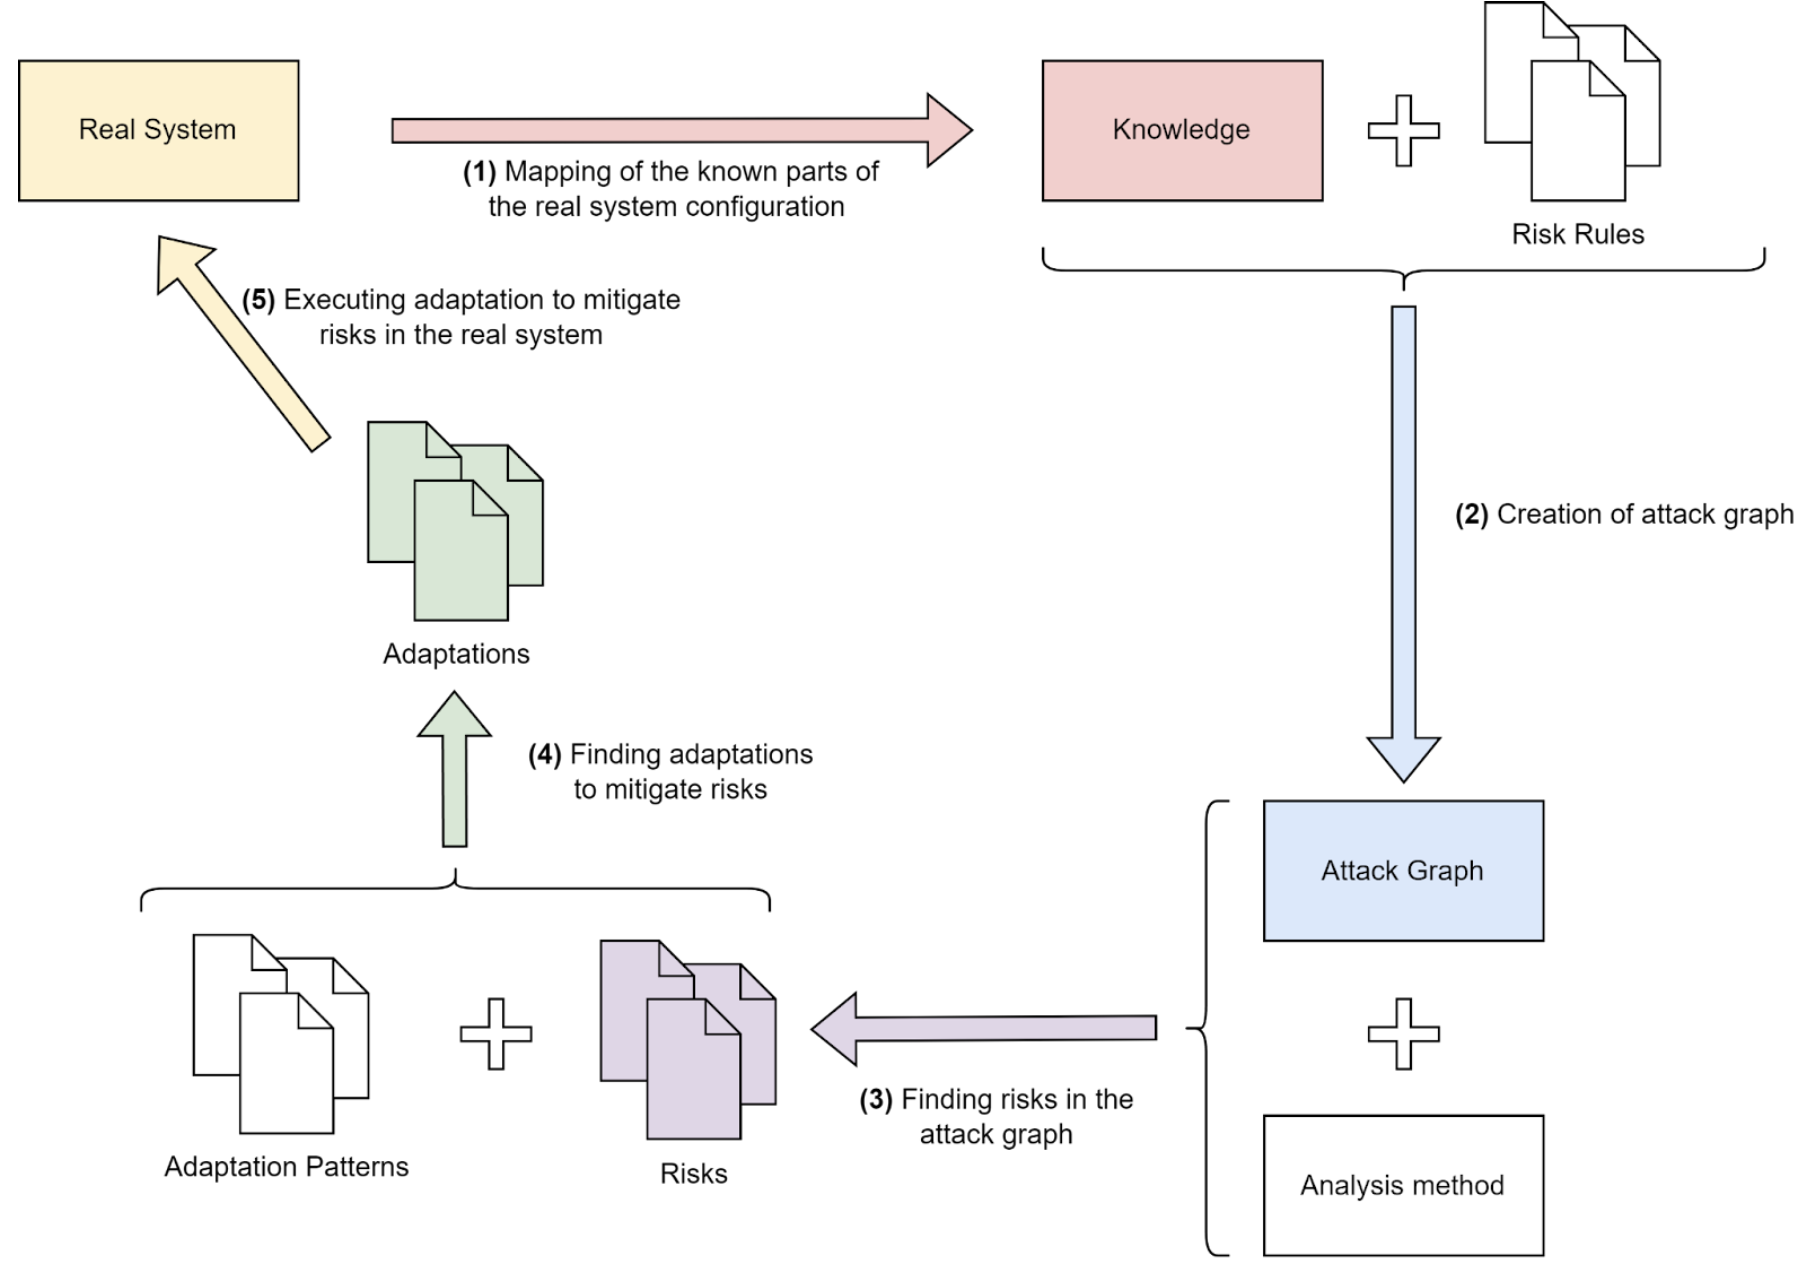
\includegraphics[width=0.8\textwidth]{content/adrian-architecture.png}
    \caption{The abstract representation of the ADRIAN approach. It shows how the different components of the system interact with each other. This figure has been sourced from the ADRIAN concept by Z.A. Mann and S. Smolka \cite{mann2023ADRIAN}.}
    \label{fig:adrian-architecture}
\end{figure}

In the ADRIAN protocol, agents are deployed across the infrastructure nodes of a system. These agents are responsible for monitoring the state of the node they are deployed on, specifically the properties of said node. These properties could range from firewall settings to OS and Firmware versions running on the node. Agents also know about the software that is deployed on their infrastructure node and its properties, such as SDK and software library versions, and if data is encrypted on disk. Knowledge about each node is then exchanged between agents, to create localized \emph{knowledge bases}.

\vspace{0.5em}
To identify risks in a network an agent uses a set of \emph{risk rules}. These risk rules are based on known vulnerabilities, which are registered in the Common Vulnerabilities and Exposures (CVEs) list\footnote{More info about CVEs can be here \url{https://www.cve.org/} }. They denote the probability of an attacker compromising the node/software. The definition of the risk rules that are implemented are detailed in section \ref{ssec:risk-rules-adaptaions}.
These risk rules are then applied to the knowledge base to create \emph{attack graphs}, which are used to reason about the risk of a network. These attack graphs serve as a dynamic representation of the system's current status, where each node is represented as a vertex and each edge represents a potential risk (CVE). It is important to note that the attack graph is not an exact reflection of the real system; rather, it is a model derived from local observations and knowledge shared among agents. 
This should be a good moment to point out that sometimes vulnerabilities and risks are not yet registered as CVEs, but could exist in the real infrastructure. This means that the attack graph is not a 100\% accurate representation of the real world system, as it is not aware of these vulnerabilities. This is a problem, as it could lead to false negatives. However, this is a problem that is not unique to the ADRIAN protocol, as it is also present in other risk detection systems.

From the attack graph, agents can derive a set of \emph{critical paths} that represent a path to a critical software component. These critical paths are then used to determine the risk of a network and the potential damage that could be done which results in a \emph{risk report}. One of these risk reports is selected and will be auctioned off to the agents in the network. In order to calculate the potential damage of a risk, the agent will combine all the probabilities of each individual edge of the attack graph along the critical path, using the following formula:

\[p = 1 - \prod_{k=1}^{R}(1-p_{k}) \]

This formula gives us a single probability per edge, which we can calculate the product of to get our final probability. This final probability is then multiplied with the critical software components damage (predetermined) to get the potential damage of the risk.

\vspace{0.5em}
The auctioning system is a mechanism that lets agents invite their peers to participate in the risk mitigation process. Once an agent has started an auction, other agents are invited to participate. These participating agents receive the risk report and attack graph as calculated by the initiating agent. Through a set of \emph{adaptation patterns}, agents can find multiple proposed solutions to reduce the potential damage of the risk report. These adaptation patterns are based on the risk rules, and describe a single adaptation that can be performed to mitigate the risk.
Each participating agent will try to select a proposal it is willing to perform. This proposal is then sent back to the auctioneer agent, which will accumulate all proposals and select the proposal that is most beneficial to the network. The selected proposal is then executed by the agent that proposed it, and the network is updated accordingly.
